% !TeX root = ../main.tex
\chapter{实验二:真实使用场景下的评测} %字符级别输入的部分
\label{cha:evaluation}
根据上一章的模拟结果,我们将半键盘的相对算法集成到了系统中,作为我们单词级别输入的模型。此外,我们还在系统中实现了字符级别输入。在本章中,我们介绍了整个系统的设计,并对单词级别输入、字符级别输入和混合模式输入三种使用场景做了用户评测。

\section{平台设计}
% 平台图以及如何进行切换
\subsection{单词级别}
在单词级别的输入中,用户和实验一相同,将双手放置于手机前,在不显示键盘的情况下,按照自己的肌肉记忆在桌面上进行十指输入。

用户在进行输入时,平台的算法会根据用户点击的位置预测出用户可能的目标单词。屏幕上会显示出现概率最高的五个单词,用户可以使用右手右滑切换目标单词,和物理键盘相似,用户通过点击空格键选择当前光标的指向单词。如果用户认为自己输入出现错误,用户可以将左手左滑删除正在输入的部分或者删除上一个输入的单词。

\subsection{字符级别}
较为直观的输入字符的方式为显示完整键盘布局,用户移动到目标字符后进行选择。然而,由于手机的屏幕相对较小,且用户输入时眼部离手机有一定距离,因此若将所有字符完整显示在屏幕上不仅瞄准相对困难,且容易造成视觉疲劳。考虑到在单词级别输入时用户使用滑动的方式进行选择,我们字符级别的输入仍然采用类似的交互思路。

总体上我们使用二级菜单的设计,如图~\ref{fig:design}。其中第一级菜单为九宫格键盘,包括了26个英文字母和3个其他字符;当用户选择第一级菜单的某个方格之后,会出现二级菜单,二级菜单显示了对应方格的字符供用户进行选择。在一二级菜单中,用户均可以使用右手右滑向右移动光标,左手左滑向左移动光标到达目标位置。仍然类似于单词输入,用户在一二级菜单进行选择时,可以使用右手任意手指进行点击。使用左手手指点击则对应退回的操作,如果当前在二级菜单则退回到一级菜单,如果在一级菜单则删除一个字符。

我们的系统支持两种模式混合输入。用户通过点击离手机较远的位置(36cm之后)切换输入模式,我们实验一的数据表明,用户在正常输入时超过30cm的点击比例小于0.1\%,且最远为32cm。另外,用户能够很容易判断如何快速点击合适位置进行切换。

\begin{figure}[htbp] % use float package if you want it here
    \centering
    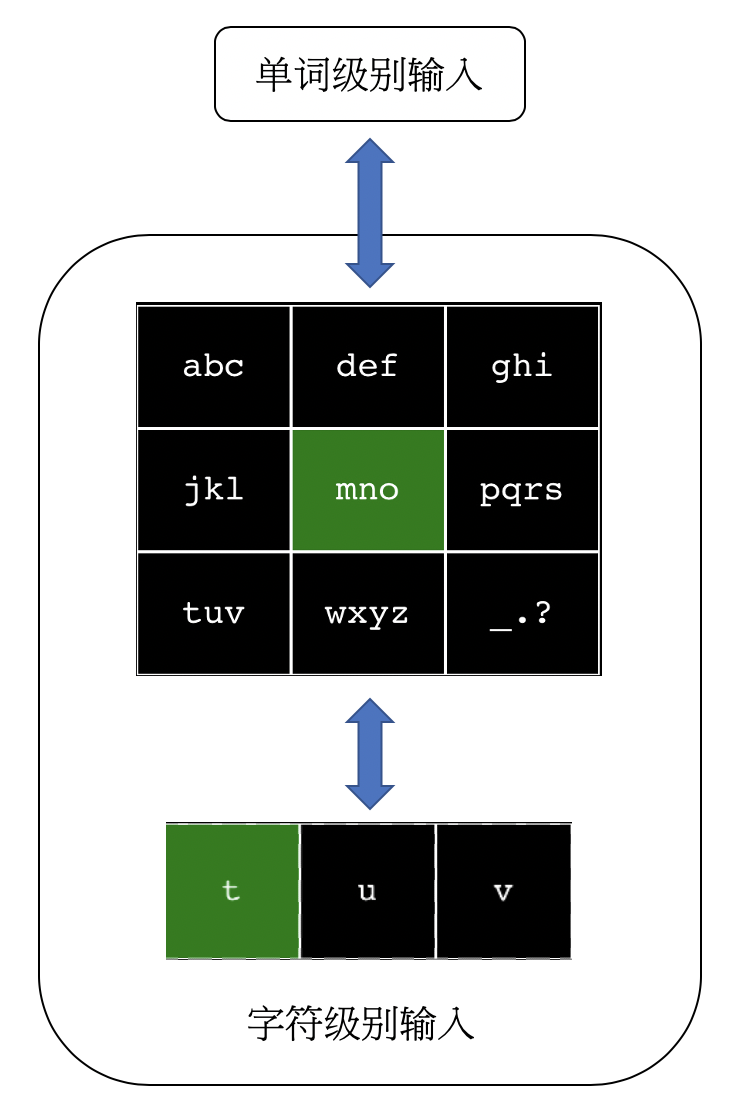
\includegraphics[height=11cm]{figures/design.png}
    \caption{平台设计结构图}
    \label{fig:design}
\end{figure}

\section{被试}
在评测实验中,我们招募了X名被试。被试们平均年龄为X岁(标准差=X),且均熟练使用实体键盘。我们仍使用了TextTest\cite{texttest}\cite{wobbrock2006analyzing}对他们物理键盘输入速度进行了测试,平均速度为单词每分钟,无纠正错误率为X\%。

\section{实验装置和实验平台}
本次实验的装置和实验一相同。实验平台同样类似,但是显示了当前的输入模式,并且多了一行单词供用户进行选择,见图~\ref{fig:platform1}。

\begin{figure}[h] % use float package if you want it here
    \centering
    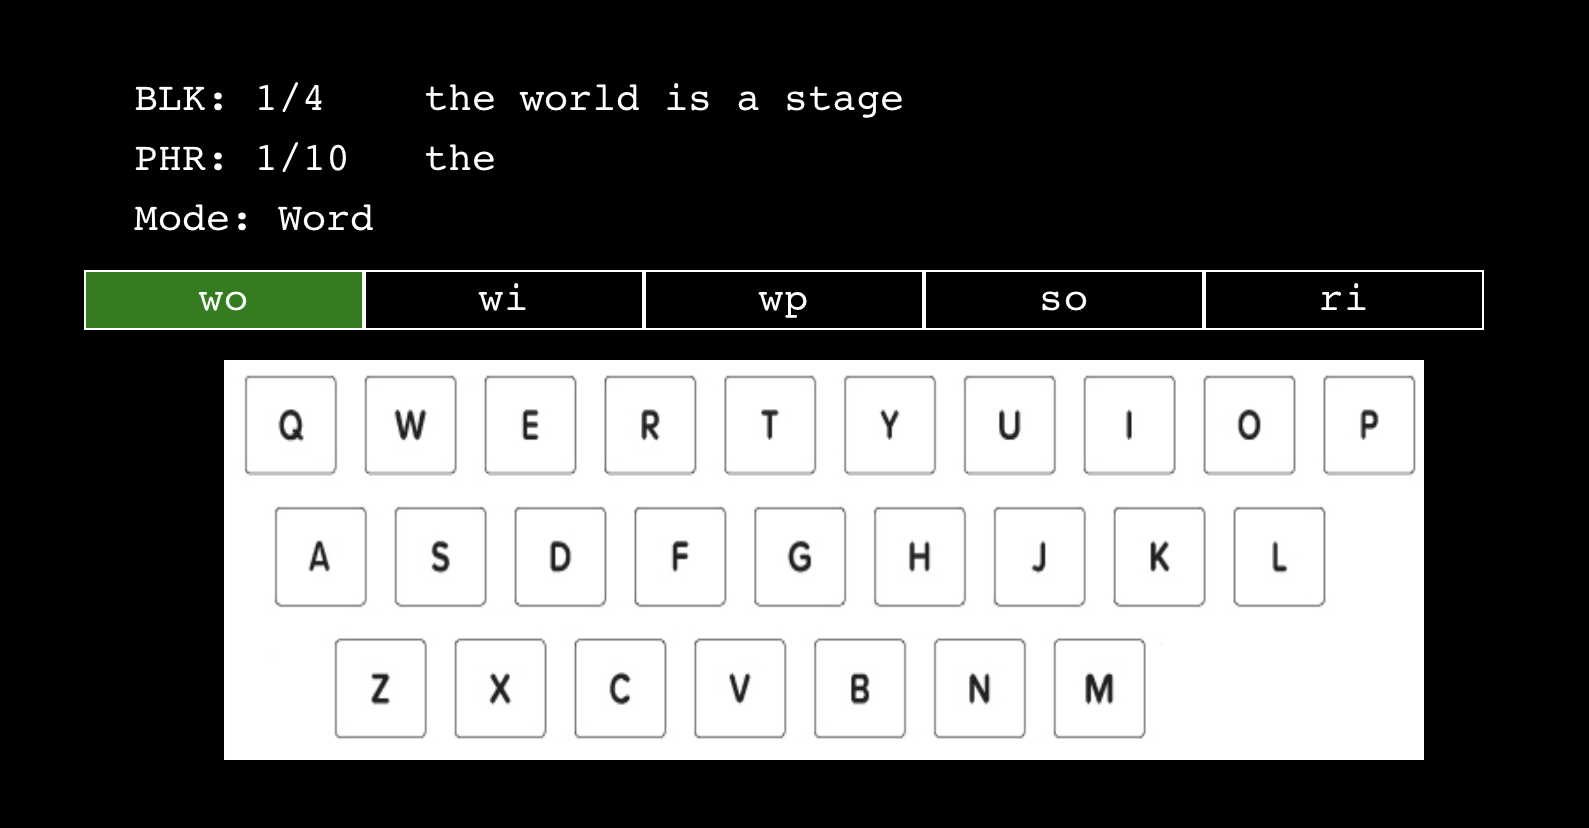
\includegraphics[height=5cm]{figures/platform1.jpg}
    \caption{实验二平台截图}
    \label{fig:platform1}
\end{figure}

\section{实验设计和流程}
为了研究我们的平台在不同情况下的输入效率,评测实验分为三个模式,分别是单词模式、字符模式和单词字符混合模式。操作方式见本章平台设计部分。为了避免不同模式顺序对结果的影响,每位用户实验时三个模式顺序随机,在屏幕上会标明当前的输入模式。在输入单词时,我们和第~\ref{cha:algorithm}~章一样,使用10,000个单词作为词库。

在正式实验开始前,每位用户有10分钟的时间熟悉实验平台。在输入时,我们要求用户尽可能快而准确进行。每当用户输入完一句话后,用户可以点击任意按键跳到下一句。在输入块之间,用户需要强制休息2分钟。在完成一句后,用户也可以根据个人需求将手放在桌面上休息。实验结束后,用户需要填写一个问卷用于收集相关信息。


\section{单词模式输入}
在单词模式的输入中,用户需要完成4个输入块,每个输入块10句话。这40句话为T-40\cite{t40}打乱而成,同样也是Mackenzie句库的子集\cite{mackenzie2003phrase}。

\subsection{输入速度}
\subsection{输入准确性}
我们使用CER\cite{cer},即字符级别准确率来衡量用户输入的准确性。CER表示将用户输入的字符串改成目标句子需要的最少的删除、增加、替换操作总次数除以目标句子长度。当CER越接近1时,则输入准确性越高。对于每个句子,我们分别计算CER,最后取平均值。

在单词输入模式中,CER整体平均值为0.15\%,四个输入块的平均值分别为0.0\%,0.6\%,0.0\%,0.0\%。总体来看,CER处于较低的水平,原因有两点,一是我们的算法准确性较高,能够预测用户的目标单词;二是即使用户点错位置或者选择了错误的单词,通常会选择重新进行输入。

\subsection{用户行为数据}
我们统计了用户在单词级别输入时的交互数据,其中“单词一匹配”表示用户选择了出现的第一个单词,且该单词与目标句子对应单词相同,“单词一不匹配”则表示选择单词一但是该单词错误;以此类推,“非单词一匹配”和“非单词一不匹配”分别表示用户选择的单词不是第一个时,该单词正确与否的情况。“撤销”操作表示用户未输入完一个单词时清空当前的输入内容;“删除”则表示用户删除输入框中一个单词,一般为选择了错误的单词后删除重新输入。

\begin{table}[h]
  \centering
  \begin{minipage}[t]{0.9\linewidth} % 如果想在表格中使用脚注,minipage是个不错的办法
  \caption[单词模式下用户各行为百分比]{单词模式下用户各行为百分比}
  \label{tab:word-stat}
    \centering
    \begin{tabularx}{\linewidth}{cccccc}
      \toprule[1.5pt]
      %  & \multicolumn{2}{c}{总体}&\multicolumn{2}{c}{左手} &  \multicolumn{2}{c}{右手} \\\midrule[1pt]
      单词一匹配 & 单词一不匹配 & 非单词一匹配 & 非单词一不匹配 & 删除 & 撤销\\\midrule[1pt]
      75.38 & 2.56 & 15.89 & 0.00 & 3.58 & 2.56\\
      \bottomrule[1.5pt]
    \end{tabularx}
  \end{minipage}
\end{table}

从表格~(\ref{tab:word-stat})可以看出,用户的绝大部分操作为“单词一匹配”(75.38\%),说明我们的算法能够很好预测用户的目标单词。不匹配的情况大部分出现在选择单词一时,表示用户输入完成一个单词直接点击确定,造成输入错误,然后用户会将该单词删除重新输入。该行为从侧面反应用户较为熟练我们的使用方法,出现类似在物理键盘上的行为。

% \section{字符模式输入}
% \section{混合模式输入}

% \section{本章总结}